%%%%%%%%%%%%%%%%%%%%%%%%%%%%%%%%%%%%%%%%%%%%%%%%%%%%%%%%%%%%%%%
%% OXFORD THESIS TEMPLATE

% Use this template to produce a standard thesis that meets the Oxford University requirements for DPhil submission
%
% Originally by Keith A. Gillow (gillow@maths.ox.ac.uk), 1997
% Modified by Sam Evans (sam@samuelevansresearch.org), 2007
% Modified by John McManigle (john@oxfordechoes.com), 2015
% Modified by Ulrik Lyngs (ulrik.lyngs@cs.ox.ac.uk), 2018-, for use with R Markdown
%
% Ulrik Lyngs, 25 Nov 2018: Following John McManigle, broad permissions are granted to use, modify, and distribute this software
% as specified in the MIT License included in this distribution's LICENSE file.
%
% John commented this file extensively, so read through to see how to use the various options.  Remember that in LaTeX,
% any line starting with a % is NOT executed.

%%%%% PAGE LAYOUT
% The most common choices should be below.  You can also do other things, like replace "a4paper" with "letterpaper", etc.

% 'twoside' formats for two-sided binding (ie left and right pages have mirror margins; blank pages inserted where needed):
%\documentclass[a4paper,twoside]{templates/ociamthesis}
% Specifying nothing formats for one-sided binding (ie left margin > right margin; no extra blank pages):
%\documentclass[a4paper]{ociamthesis}
% 'nobind' formats for PDF output (ie equal margins, no extra blank pages):
%\documentclass[a4paper,nobind]{templates/ociamthesis}

% As you can see from the line below, oxforddown uses the a4paper size, 
% and passes in the binding option from the YAML header in index.Rmd:
\documentclass[a4paper, nobind]{templates/ociamthesis}


%%%%% ADDING LATEX PACKAGES
% add hyperref package with options from YAML %
\usepackage[pdfpagelabels]{hyperref}
% handle long urls
\usepackage{xurl}
% change the default coloring of links to something sensible
\usepackage{xcolor}

\definecolor{mylinkcolor}{RGB}{0,0,139}
\definecolor{myurlcolor}{RGB}{0,0,139}
\definecolor{mycitecolor}{RGB}{0,33,71}

\hypersetup{
  hidelinks,
  colorlinks,
  linktocpage=true,
  linkcolor=mylinkcolor,
  urlcolor=myurlcolor,
  citecolor=mycitecolor
}


% add float package to allow manual control of figure positioning %
\usepackage{float}

% enable strikethrough
\usepackage[normalem]{ulem}

% use soul package for correction highlighting
\usepackage{color, soul}
\definecolor{correctioncolor}{HTML}{CCCCFF}
\sethlcolor{correctioncolor}
\newcommand{\ctext}[3][RGB]{%
  \begingroup
  \definecolor{hlcolor}{#1}{#2}\sethlcolor{hlcolor}%
  \hl{#3}%
  \endgroup
}
% stop soul from freaking out when it sees citation commands
\soulregister\ref7
\soulregister\cite7
\soulregister\citet7
\soulregister\autocite7
\soulregister\textcite7
\soulregister\pageref7

%%%%% FIXING / ADDING THINGS THAT'S SPECIAL TO R MARKDOWN'S USE OF LATEX TEMPLATES
% pandoc puts lists in 'tightlist' command when no space between bullet points in Rmd file,
% so we add this command to the template
\providecommand{\tightlist}{%
  \setlength{\itemsep}{0pt}\setlength{\parskip}{0pt}}
 
% allow us to include code blocks in shaded environments
\usepackage{color}
\usepackage{fancyvrb}
\newcommand{\VerbBar}{|}
\newcommand{\VERB}{\Verb[commandchars=\\\{\}]}
\DefineVerbatimEnvironment{Highlighting}{Verbatim}{commandchars=\\\{\}}
% Add ',fontsize=\small' for more characters per line
\usepackage{framed}
\definecolor{shadecolor}{RGB}{248,248,248}
\newenvironment{Shaded}{\begin{snugshade}}{\end{snugshade}}
\newcommand{\AlertTok}[1]{\textcolor[rgb]{0.94,0.16,0.16}{#1}}
\newcommand{\AnnotationTok}[1]{\textcolor[rgb]{0.56,0.35,0.01}{\textbf{\textit{#1}}}}
\newcommand{\AttributeTok}[1]{\textcolor[rgb]{0.13,0.29,0.53}{#1}}
\newcommand{\BaseNTok}[1]{\textcolor[rgb]{0.00,0.00,0.81}{#1}}
\newcommand{\BuiltInTok}[1]{#1}
\newcommand{\CharTok}[1]{\textcolor[rgb]{0.31,0.60,0.02}{#1}}
\newcommand{\CommentTok}[1]{\textcolor[rgb]{0.56,0.35,0.01}{\textit{#1}}}
\newcommand{\CommentVarTok}[1]{\textcolor[rgb]{0.56,0.35,0.01}{\textbf{\textit{#1}}}}
\newcommand{\ConstantTok}[1]{\textcolor[rgb]{0.56,0.35,0.01}{#1}}
\newcommand{\ControlFlowTok}[1]{\textcolor[rgb]{0.13,0.29,0.53}{\textbf{#1}}}
\newcommand{\DataTypeTok}[1]{\textcolor[rgb]{0.13,0.29,0.53}{#1}}
\newcommand{\DecValTok}[1]{\textcolor[rgb]{0.00,0.00,0.81}{#1}}
\newcommand{\DocumentationTok}[1]{\textcolor[rgb]{0.56,0.35,0.01}{\textbf{\textit{#1}}}}
\newcommand{\ErrorTok}[1]{\textcolor[rgb]{0.64,0.00,0.00}{\textbf{#1}}}
\newcommand{\ExtensionTok}[1]{#1}
\newcommand{\FloatTok}[1]{\textcolor[rgb]{0.00,0.00,0.81}{#1}}
\newcommand{\FunctionTok}[1]{\textcolor[rgb]{0.13,0.29,0.53}{\textbf{#1}}}
\newcommand{\ImportTok}[1]{#1}
\newcommand{\InformationTok}[1]{\textcolor[rgb]{0.56,0.35,0.01}{\textbf{\textit{#1}}}}
\newcommand{\KeywordTok}[1]{\textcolor[rgb]{0.13,0.29,0.53}{\textbf{#1}}}
\newcommand{\NormalTok}[1]{#1}
\newcommand{\OperatorTok}[1]{\textcolor[rgb]{0.81,0.36,0.00}{\textbf{#1}}}
\newcommand{\OtherTok}[1]{\textcolor[rgb]{0.56,0.35,0.01}{#1}}
\newcommand{\PreprocessorTok}[1]{\textcolor[rgb]{0.56,0.35,0.01}{\textit{#1}}}
\newcommand{\RegionMarkerTok}[1]{#1}
\newcommand{\SpecialCharTok}[1]{\textcolor[rgb]{0.81,0.36,0.00}{\textbf{#1}}}
\newcommand{\SpecialStringTok}[1]{\textcolor[rgb]{0.31,0.60,0.02}{#1}}
\newcommand{\StringTok}[1]{\textcolor[rgb]{0.31,0.60,0.02}{#1}}
\newcommand{\VariableTok}[1]{\textcolor[rgb]{0.00,0.00,0.00}{#1}}
\newcommand{\VerbatimStringTok}[1]{\textcolor[rgb]{0.31,0.60,0.02}{#1}}
\newcommand{\WarningTok}[1]{\textcolor[rgb]{0.56,0.35,0.01}{\textbf{\textit{#1}}}}

% set white space before and after code blocks


\renewenvironment{Shaded}
{
  \vspace{10pt}%
  \begin{snugshade}%
}{%
  \end{snugshade}%
  \vspace{8pt}%
}

% User-included things with header_includes or in_header will appear here
% kableExtra packages will appear here if you use library(kableExtra)
\usepackage{fontspec}
\setmainfont{Arial}
\usepackage{booktabs}
\usepackage{longtable}
\usepackage{array}
\usepackage{multirow}
\usepackage{wrapfig}
\usepackage{float}
\usepackage{colortbl}
\usepackage{pdflscape}
\usepackage{tabu}
\usepackage{threeparttable}
\usepackage{threeparttablex}
\usepackage[normalem]{ulem}
\usepackage{makecell}
\usepackage{xcolor}


%UL set section header spacing
\usepackage{titlesec}
% 
\titlespacing\subsubsection{0pt}{24pt plus 4pt minus 2pt}{0pt plus 2pt minus 2pt}


%UL set whitespace around verbatim environments
\usepackage{etoolbox}
\makeatletter
\preto{\@verbatim}{\topsep=0pt \partopsep=0pt }
\makeatother


%%%%%%% PAGE HEADERS AND FOOTERS %%%%%%%%%
\usepackage{fancyhdr}
\setlength{\headheight}{15pt}
\fancyhf{} % clear the header and footers
\pagestyle{fancy}
\renewcommand{\chaptermark}[1]{\markboth{\thechapter. #1}{\thechapter. #1}}
\renewcommand{\sectionmark}[1]{\markright{\thesection. #1}} 
\renewcommand{\headrulewidth}{0pt}

\fancyhead[LO]{\emph{\leftmark}} 
\fancyhead[RE]{\emph{\rightmark}} 




% UL page number position 
\fancyhead[R]{\emph{\thepage}} %regular pages
\fancypagestyle{plain}{\fancyhf{}\fancyfoot[L]{\emph{\thepage}}} %chapter pages




%%%%% SELECT YOUR DRAFT OPTIONS
% This adds a "DRAFT" footer to every normal page.  (The first page of each chapter is not a "normal" page.)

% IP feb 2021: option to include line numbers in PDF

% for line wrapping in code blocks
\usepackage{fancyvrb}
\usepackage{fvextra}
\DefineVerbatimEnvironment{Highlighting}{Verbatim}{breaklines=true, breakanywhere=true, commandchars=\\\{\}}

% for quotations -- loaded here rather than in ociamthesis.cls, as it needs to
% be loaded after fvextra, otherwise we get a warning message
\usepackage{csquotes}

% This highlights (in blue) corrections marked with (for words) \mccorrect{blah} or (for whole
% paragraphs) \begin{mccorrection} . . . \end{mccorrection}.  This can be useful for sending a PDF of
% your corrected thesis to your examiners for review.  Turn it off, and the blue disappears.
\correctionstrue


%%%%% BIBLIOGRAPHY SETUP
% Note that your bibliography will require some tweaking depending on your department, preferred format, etc.
% If you've not used LaTeX before, I recommend just using pandoc for citations -- this is what's used unless you specific e.g. "citation_package: natbib" in index.Rmd
% If you're already a LaTeX pro and are used to natbib or something, modify as necessary.

% this allows the latex template to handle pandoc citations
\newlength{\cslhangindent}
\setlength{\cslhangindent}{1.5em}
\newlength{\csllabelwidth}
\setlength{\csllabelwidth}{3em}
\newlength{\cslentryspacingunit} % times entry-spacing
\setlength{\cslentryspacingunit}{\parskip}
\newenvironment{CSLReferences}[2] % #1 hanging-ident, #2 entry spacing
 {% don't indent paragraphs
  \setlength{\parindent}{0pt}
  % turn on hanging indent if param 1 is 1
  \ifodd #1
  \let\oldpar\par
  \def\par{\hangindent=\cslhangindent\oldpar}
  \fi
  % set entry spacing
  \setlength{\parskip}{1mm}
  \setlength{\baselineskip}{6mm}
 }%
 {}
\usepackage{calc}
\newcommand{\CSLBlock}[1]{#1\hfill\break}
\newcommand{\CSLLeftMargin}[1]{\parbox[t]{\csllabelwidth}{#1}}
\newcommand{\CSLRightInline}[1]{\parbox[t]{\linewidth - \csllabelwidth}{#1}\break}
\newcommand{\CSLIndent}[1]{\hspace{\cslhangindent}#1}




% Uncomment this if you want equation numbers per section (2.3.12), instead of per chapter (2.18):
%\numberwithin{equation}{subsection}


%%%%% THESIS / TITLE PAGE INFORMATION
% Everybody needs to complete the following:
\title{Analisis Ekonomi dan Keuangan\\
dengan \texttt{RStudio}\\}
\author{Tedy Herlambang}
\college{---}

% Master's candidates who require the alternate title page (with candidate number and word count)
% must also un-comment and complete the following three lines:

% Uncomment the following line if your degree also includes exams (eg most masters):
%\renewcommand{\submittedtext}{Submitted in partial completion of the}
% Your full degree name.  (But remember that DPhils aren't "in" anything.  They're just DPhils.)
\degree{---}

% Term and year of submission, or date if your board requires (eg most masters)
\degreedate{----}


%%%%% YOUR OWN PERSONAL MACROS
% This is a good place to dump your own LaTeX macros as they come up.

% To make text superscripts shortcuts
\renewcommand{\th}{\textsuperscript{th}} % ex: I won 4\th place
\newcommand{\nd}{\textsuperscript{nd}}
\renewcommand{\st}{\textsuperscript{st}}
\newcommand{\rd}{\textsuperscript{rd}}

%%%%% THE ACTUAL DOCUMENT STARTS HERE
\begin{document}

%%%%% CHOOSE YOUR LINE SPACING HERE
% This is the official option.  Use it for your submission copy and library copy:
\setlength{\textbaselineskip}{22pt plus2pt}
% This is closer spacing (about 1.5-spaced) that you might prefer for your personal copies:
%\setlength{\textbaselineskip}{18pt plus2pt minus1pt}

% You can set the spacing here for the roman-numbered pages (acknowledgements, table of contents, etc.)
\setlength{\frontmatterbaselineskip}{17pt plus1pt minus1pt}

% UL: You can set the line and paragraph spacing here for the separate abstract page to be handed in to Examination schools
\setlength{\abstractseparatelineskip}{13pt plus1pt minus1pt}
\setlength{\abstractseparateparskip}{0pt plus 1pt}

% UL: You can set the general paragraph spacing here - I've set it to 2pt (was 0) so
% it's less claustrophobic
\setlength{\parskip}{2pt plus 1pt}

%
% Customise title page
%
\def\crest{}
\renewcommand{\university}{---}
\renewcommand{\submittedtext}{---}
\renewcommand{\thesistitlesize}{\fontsize{22pt}{28pt}\selectfont}
\renewcommand{\gapbeforecrest}{25mm}
\renewcommand{\gapaftercrest}{25mm
}


% Leave this line alone; it gets things started for the real document.
\setlength{\baselineskip}{\textbaselineskip}


%%%%% CHOOSE YOUR SECTION NUMBERING DEPTH HERE
% You have two choices.  First, how far down are sections numbered?  (Below that, they're named but
% don't get numbers.)  Second, what level of section appears in the table of contents?  These don't have
% to match: you can have numbered sections that don't show up in the ToC, or unnumbered sections that
% do.  Throughout, 0 = chapter; 1 = section; 2 = subsection; 3 = subsubsection, 4 = paragraph...

% The level that gets a number:
\setcounter{secnumdepth}{2}
% The level that shows up in the ToC:
\setcounter{tocdepth}{1}


%%%%% ABSTRACT SEPARATE
% This is used to create the separate, one-page abstract that you are required to hand into the Exam
% Schools.  You can comment it out to generate a PDF for printing or whatnot.

% JEM: Pages are roman numbered from here, though page numbers are invisible until ToC.  This is in
% keeping with most typesetting conventions.
\begin{romanpages}

% Title page is created here
\maketitle

%%%%% DEDICATION
\begin{dedication}
  Untuk Para Pengembang \texttt{R\ Markdown} dan \texttt{Bookdown}
\end{dedication}

%%%%% ACKNOWLEDGEMENTS


\begin{acknowledgements}
 	Terima kasih yang sebesar-besarnya saya sampaikan kepada: Prof.~Abdul Haris, Dr.~Titik Musriati dan Dr.~Ngatimun (Universitas Panca Marga), Muhammad Agus Nugroho dan Rifaldi Kadir (UIN Gorontalo), Rudi Masniadi (Universitas Teknologi Sumbawa), Erlyn Yuniashri dan Ajeng Kartika Galuh (Universitas Brawijaya Malang), Oktaviani Ika Wijayanti, Frederic Winston Nalle (Universitas Timor), Yeni Puspita (Universitas Negeri Jember) dan Muhammad Rizal (Universitas Islam Malang).

 \begin{flushright}
 Tedy Herlambang \\
 UPM \\
 4 Januari 2024
 \end{flushright}
\end{acknowledgements}



%%%%% ABSTRACT


\renewcommand{\abstracttitle}{Sinopsis}
\begin{abstract}
	Buku ini merupakan \emph{pengantar} cara melakukan analisis ekonomi dan bisnis secara kuantitatif dengan menggunakan R dan RStudio. Persoalan yang dibahas umumnya tingkat S1 atau S2.

Saya berharap pembaca dapat mengambil satu gagasan dari buku ini dalam melakukan investigasi ekonomi dan bisnis secara kuantitatif: data dan alat-alat analisis tidak sempurna. Namun, ketika kita memahami kekuatan dan kelemahan alat-alat ini, kita dapat menggunakannya untuk menemukan hal-hal menarik di dalam ekonomi dan bisnis.

Jangan ragu untuk menghubungi saya dengan pemikiran Anda tentang buku ini, ide perbaikan/materi tambahan atau mungkin kesalahan yang Anda temukan di buku ini.
\end{abstract}



%%%%% MINI TABLES
% This lays the groundwork for per-chapter, mini tables of contents.  Comment the following line
% (and remove \minitoc from the chapter files) if you don't want this.  Un-comment either of the
% next two lines if you want a per-chapter list of figures or tables.
\dominitoc % include a mini table of contents

% This aligns the bottom of the text of each page.  It generally makes things look better.
\flushbottom

% This is where the whole-document ToC appears:
\tableofcontents

\listoffigures
	\mtcaddchapter
  	% \mtcaddchapter is needed when adding a non-chapter (but chapter-like) entity to avoid confusing minitoc

% Uncomment to generate a list of tables:
\listoftables
  \mtcaddchapter
%%%%% LIST OF ABBREVIATIONS
% This example includes a list of abbreviations.  Look at text/abbreviations.tex to see how that file is
% formatted.  The template can handle any kind of list though, so this might be a good place for a
% glossary, etc.
% First parameter can be changed eg to "Glossary" or something.
% Second parameter is the max length of bold terms.
\begin{mclistof}{Daftar Istilah}{3.2cm}

\item[1-D, 2-D]

\begin{center}\rule{0.5\linewidth}{0.5pt}\end{center}

\item[Otter]

\begin{center}\rule{0.5\linewidth}{0.5pt}\end{center}

\item[Hedgehog]

\begin{center}\rule{0.5\linewidth}{0.5pt}\end{center}

\end{mclistof} 


% The Roman pages, like the Roman Empire, must come to its inevitable close.
\end{romanpages}

%%%%% CHAPTERS
% Add or remove any chapters you'd like here, by file name (excluding '.tex'):
\flushbottom

% all your chapters and appendices will appear here
\hypertarget{pengenalan-r-dan-rstudio}{%
\chapter{Pengenalan R dan RStudio}\label{pengenalan-r-dan-rstudio}}

\minitoc 

Alat utama yang akan kita gunakan untuk analisis ekonomi dan keuangan dalam buku ini adalah \texttt{R} (Team (\protect\hyperlink{ref-rcoreteamLanguageEnvironmentStatistical2023}{2023})) dan \href{https://posit.co/download/rstudio-desktop/}{\texttt{RStudio}}. RStudio bukan R, juga tidak menyertakan R saat Anda mengunduh dan menginstalnya. Oleh karena itu, R dan RStudio perlu diunduh dan diinstal terpisah.

R dapat diunduh di \href{http://www.r-project.org/}{R Project for Statistical Computing}. Di situs ini juga terdapat tautan ke buku, manual, \emph{R Journal} dan lain-lain untuk belajar R. Silakan unduh R di situs ini sesuai dengan platform komputasi Anda Windows, Macintosh atau Unix. Gratis! Sedangkan untuk menginstal RStudio silakan kunjungi \href{https://posit.co/download/rstudio-desktop/}{posit}. Silakan unduh \emph{RStudio Desktop} dari situs ini. Juga gratis! Untuk pengenalan ini, saya berasumsi bahwa Anda telah mengunduh dan menginstal R dan RStudio di komputer Anda.

R tidak punya pengembang antarmuka pengguna grafis (GUI) yang sesuai dengan keinginan pengguna seperti halnya program SPSS atau Stata. GUI bawaan R terlihat lebih mirip dengan konsol DOS lama (lihat Gambar \ref{fig:rgui}). Oleh karena itu, dalam buku ini kita akan fokus menggunakan R melalui antarmuka \emph{RStudio}. Dengan RStudio, R lebih mudah digunakan dan lebih mirip dengan program SPSS atau Stata.

\begin{figure}[H]
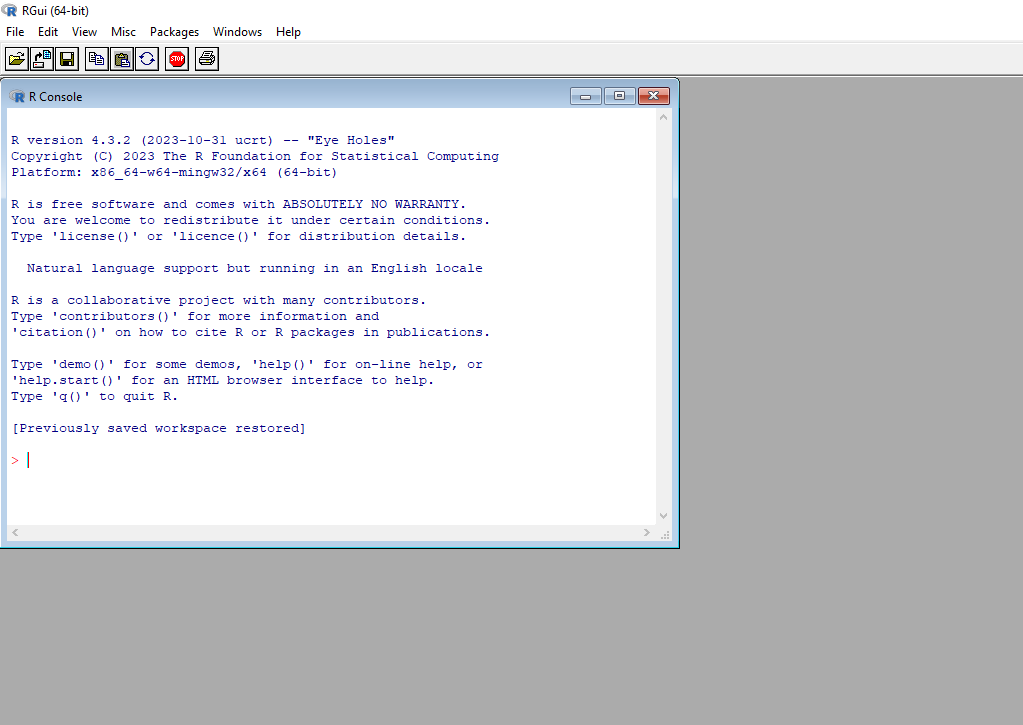
\includegraphics[width=1\linewidth]{figures/console432} \caption{GUI R}\label{fig:rgui}
\end{figure}

Hubungan antara R dan RStudio seperti mesin mobil dan dashboard (Ismay \& Kim (\protect\hyperlink{ref-ismayStatisticalInferenceData2019}{2019})). Bahasa R dapat diumpamakan sebagai mesin mobil, sedangkan RStudio sebagai dasbornya sehingga kita mudah mengkonfigurasi dan mengontrol kerja mesin.

Di buku ini, saya tidak menunjukkan fitur-fitur R dan RStudio yang sangat banyak secara mendetil. Bab ini hanya berisi contoh mengoperasikan R dan RStudio, metode untuk menginstal paket R dan paket pihak ketiga yang diperlukan untuk digunakan dalam buku ini di bab berikutnya.

\hypertarget{tata-letak-rstudio}{%
\section{Tata Letak RStudio}\label{tata-letak-rstudio}}

Sebagai permulaan, kita akan mempelajari tata letak RStudio dan elemen inti yang akan kita gunakan. Saat Anda memulai RStudio untuk pertama kalinya, Anda akan melihat tiga panel (lihat Gambar \ref{fig:3qu}).

\begin{enumerate}
\def\labelenumi{\arabic{enumi}.}
\tightlist
\item
  Panel kiri menunjukkan konsol R. Panel ini seperti GUI R yang kita lihat sebelumnnya. Di panel ini kita bisa mengetikkan perintah untuk R.
\item
  Panel kanan atas berisi lima tab: \emph{Environment, History, Connections, Build} dan \emph{Tutorial}. Di dalam Environment semua kumpulan data, variabel, model, objek, dan plot akan disimpan.
\item
  Panel kanan bawah menampilkan enam tab: \emph{File, Plots, Packages, Help, Viewer} dan \emph{Presentation}. Tab \emph{Plots} adalah tempat mencetak atau mengekspor plot dan grafik. Tab \emph{Packages} menunjukkan berbagai paket yang terpasang di komputer Anda. Tab yang penting disini adalah \emph{Help}: kita bisa mencari informasi jika kita lupa dengan fungsi-fungsi tertentu di dalam R. Anda dapat mengklik setiap tab untuk menelusuri berbagai fitur di dalamnya.
\end{enumerate}

\begin{figure}[H]
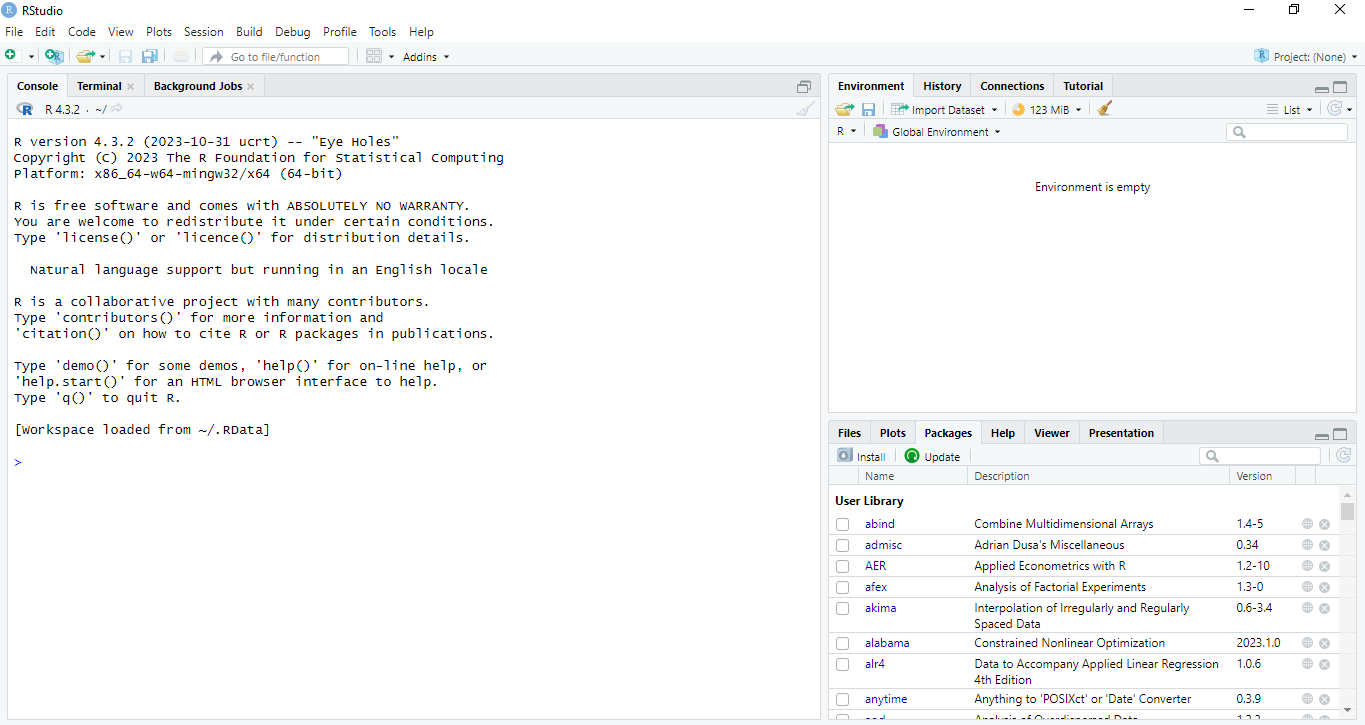
\includegraphics[width=1\linewidth]{figures/3qu} \caption{Antar Muka RStudio}\label{fig:3qu}
\end{figure}

\hypertarget{membuat-projek}{%
\section{Membuat Projek}\label{membuat-projek}}

Setelah Anda membuka RStudio, langkah pertama yang sebaiknya Anda lakukan adalah membuat file projek. Sebuah projek adalah tempat terpusat untuk semua objek, grafik dan skrip untuk projek kita. Dengan membuat projek, kita tidak perlu memikirkan lagi direktori kerja untuk menyimpan perhitungan, file, history dan data. Semua akan disimpan di dalam folder projek ini.

Folder projek ini dapat disamakan dengan folder fisik tempat Anda menyimpan riset topik tertentu (misal projek \emph{economic growth}, \emph{game theory}, \emph{financial engineering}). Masing-masing projek harus dibuatkan folder terpisah. Saat Anda ingin mengerjakan projek, Anda membuka folder Anda (dan menutup projek Anda setelah selesai). Saat kembali, Anda dapat membuka kembali folder dan melanjutkan dari bagian terakhir yang Anda tinggalkan. Projek RStudio juga serupa dalam hal itu.

Langkah-langkah untuk membuat sebuah projek adalah:

\begin{enumerate}
\def\labelenumi{\arabic{enumi}.}
\tightlist
\item
  Di RStudio pilih ``File'' lalu ``New Project.'' Atau klik tanda R di pojok kanan atas, kemudian ``New Project''.
\item
  Selanjutnya pilih opsi pertama ``New Directory'' - ini akan membuat folder baru di komputer Anda.
\item
  Di tahap berikutnya pilih ``New Directory'' atau ``Existing Directory''. Tergantung pada opsi yang Anda pilih, Anda akan memiliki beberapa pilihan di mana Anda ingin menempatkan proyek ini.
\item
  Selanjutnya beri nama projek sesuka Anda.
\item
  Klik tombol ``Create Project''.
\end{enumerate}

\hypertarget{r-dalam-gaya-tanya-jawab}{%
\section{R dalam Gaya ``Tanya Jawab''}\label{r-dalam-gaya-tanya-jawab}}

Kita dapat menggunakan R secara interaktif atau R dalam gaya ``tanya jawab'' (Dalgaard (\protect\hyperlink{ref-dalgaardIntroductoryStatistics2008}{2008})). Caranya dengan mengetik langsung di konsol panel di sebelah kiri (lihat Gambar \ref{fig:3qu}). Kita menggunakan gaya ini ketika hanya penghitungan rumus tunggal yang diperlukan.

Konsol R dapat digunakan seperti kalkulator sederhana. Mengetik ekspresi matematika dan menekan Enter akan mencetak hasilnya. Sebagai ilustrasi, misalnya Anda ingin menghitung 1 + 2, kita tulis setelah \textbf{\textgreater{}} \emph{1+2} dan tekan \textbf{Enter}. Hasilnya tigakan? Urutan aturan operasi berlaku dan banyak fungsi matematika lain seperti akar kuadrat, \texttt{sqrt}, juga dapat diterapkan seperti yang diperlihatkan di contoh berikutnya.

\begin{Shaded}
\begin{Highlighting}[]
\DecValTok{1}\SpecialCharTok{+}\DecValTok{2}
\end{Highlighting}
\end{Shaded}

\begin{verbatim}
## [1] 3
\end{verbatim}

\begin{Shaded}
\begin{Highlighting}[]
\DecValTok{1} \SpecialCharTok{/}\NormalTok{ (}\DecValTok{2} \SpecialCharTok{+} \DecValTok{15}\NormalTok{) }\SpecialCharTok{{-}} \FloatTok{1.5} \SpecialCharTok{+} \FunctionTok{sqrt}\NormalTok{(}\DecValTok{3}\NormalTok{)}
\end{Highlighting}
\end{Shaded}

\begin{verbatim}
## [1] 0.2908743
\end{verbatim}

Selanjutnya kita mungkin ingin memberi nama dan menyimpan hasil perhitungan sebagai variabel, misalnya \emph{tilu}. Maka kita tuliskan \texttt{tilu\ \textless{}-\ 1+2}. Artinya komputer menghitung 1 + 2 dan menyimpan hasilnya dalam variabel bernama tilu Pada saat kita mengetikkan \texttt{tilu\ \textless{}-\ 1+2}, dan menekan Enter, seolah-olah tidak terjadi apa-apa pada RStudio. Maka untuk memanggil variabel tilu kita ketikkan lagi tilu dan tekan Enter. Perhatikan operator penugasan \textbf{\textless-} sebagai ciri khas R, walaupun kita bisa juga menggunakan tanda =. Perhatikan di buku ini perintah ditampilkan dalam kotak abu-abu, sedangkan luarannya didahului dengan tanda pagar ganda \#\#. Dengan cara yang sama kita membuat variabel \texttt{opat\ =\ 2+2}.

\begin{Shaded}
\begin{Highlighting}[]
\NormalTok{tilu }\OtherTok{\textless{}{-}} \DecValTok{1}\SpecialCharTok{+}\DecValTok{2}
\NormalTok{tilu }\CommentTok{\# memanggil variabel opat}
\end{Highlighting}
\end{Shaded}

\begin{verbatim}
## [1] 3
\end{verbatim}

\begin{Shaded}
\begin{Highlighting}[]
\NormalTok{opat }\OtherTok{=} \DecValTok{2}\SpecialCharTok{+}\DecValTok{2}
\NormalTok{opat}
\end{Highlighting}
\end{Shaded}

\begin{verbatim}
## [1] 4
\end{verbatim}

Setelah kita mendefinisikan suatu variabel, kita dapat melakukan perhitungan lanjutan dengan variabel tersebut. Di dalam penelitian ekonomi dan keuangan hal ini sering kita lakukan misalnya menghitung \emph{return} saham, GDP perkapita, inflasi dan lain-lain, yang baru bisa kita dapatkan setelah melakukan penghitungan lanjutan dari data mentah yang didapat.

\begin{Shaded}
\begin{Highlighting}[]
\NormalTok{opat}\SpecialCharTok{\^{}}\DecValTok{2} \CommentTok{\# variabel opat dikuadratkan}
\end{Highlighting}
\end{Shaded}

\begin{verbatim}
## [1] 16
\end{verbatim}

\begin{Shaded}
\begin{Highlighting}[]
\FunctionTok{log}\NormalTok{(tilu) }\CommentTok{\#variabel tilu dilogaritma}
\end{Highlighting}
\end{Shaded}

\begin{verbatim}
## [1] 1.098612
\end{verbatim}

Operasi lain yang bisa dilakukan antara lain aritmatika (+, -, /, \^{},\ldots), operator perbandingan (==, \textless=,\ldots), operator logika (\&, \textbar, !,\ldots) dan fungsi matematika dasar seperti sin, cos, exp dan sqrt.

\hypertarget{vektor}{%
\section{Vektor}\label{vektor}}

Variabel paling dasar dalam R adalah vektor. Vektor R adalah barisan nilai yang bertipe sama. Misalnya, untuk membuat vektor lima dimensi beranggotakan angka 10, dan kita beri nama \emph{lima10}, maka ketikkan \texttt{lima10\ \textless{}-rep(10,5)} di konsol dan tekan Enter. Maka lima10 adalah vektor dengan lima elemen masing-masing 10; untuk melihatnya kita ketik \texttt{lima10} dan tekan Enter. Fungsi \emph{rep} merupakan fungsi khusus dari R yang merupakan kependekan dari pengulangan (repeat). Argumennya ditulis sebagai \emph{rep(apa yang diulang, berapa kali pengulangan)}.

\begin{Shaded}
\begin{Highlighting}[]
\NormalTok{lima10 }\OtherTok{\textless{}{-}}\FunctionTok{rep}\NormalTok{(}\DecValTok{10}\NormalTok{,}\DecValTok{5}\NormalTok{)}
\NormalTok{lima10}
\end{Highlighting}
\end{Shaded}

\begin{verbatim}
## [1] 10 10 10 10 10
\end{verbatim}

Jika a dan b bilangan bulat, perintah a:b akan membuat vektor bilangan bulat dari a ke b.

\begin{Shaded}
\begin{Highlighting}[]
\NormalTok{vektor17 }\OtherTok{\textless{}{-}} \DecValTok{1}\SpecialCharTok{:}\DecValTok{7}
\NormalTok{vektor17}
\end{Highlighting}
\end{Shaded}

\begin{verbatim}
## [1] 1 2 3 4 5 6 7
\end{verbatim}

Untuk lebih bisa mengontrol vektor yang dibuat, Anda gunakan perintah \texttt{seq}.

\begin{Shaded}
\begin{Highlighting}[]
\NormalTok{sek305 }\OtherTok{\textless{}{-}} \FunctionTok{seq}\NormalTok{(}\DecValTok{1}\NormalTok{,}\DecValTok{30}\NormalTok{,}\DecValTok{5}\NormalTok{) }\CommentTok{\# membuat vektor bilangan dari 1{-}30 dengan beda 5}
\NormalTok{sek305}
\end{Highlighting}
\end{Shaded}

\begin{verbatim}
## [1]  1  6 11 16 21 26
\end{verbatim}

\begin{Shaded}
\begin{Highlighting}[]
\NormalTok{sek301 }\OtherTok{\textless{}{-}} \FunctionTok{seq}\NormalTok{(}\DecValTok{30}\NormalTok{,}\DecValTok{1}\NormalTok{,}\SpecialCharTok{{-}}\DecValTok{5}\NormalTok{) }\CommentTok{\# membuat vektor bilangan dari 30{-}1 dengan beda {-}5}
\NormalTok{sek301}
\end{Highlighting}
\end{Shaded}

\begin{verbatim}
## [1] 30 25 20 15 10  5
\end{verbatim}

Elemen vektor dapat diindeks dengan tanda kurung {[} {]}. Argumen braket dapat berupa bilangan bulat tunggal atau vektor.

\begin{Shaded}
\begin{Highlighting}[]
\NormalTok{sek305[}\DecValTok{4}\NormalTok{]}
\end{Highlighting}
\end{Shaded}

\begin{verbatim}
## [1] 16
\end{verbatim}

\begin{Shaded}
\begin{Highlighting}[]
\NormalTok{sek305[}\DecValTok{1}\SpecialCharTok{:}\DecValTok{4}\NormalTok{]}
\end{Highlighting}
\end{Shaded}

\begin{verbatim}
## [1]  1  6 11 16
\end{verbatim}

\begin{Shaded}
\begin{Highlighting}[]
\NormalTok{sek305[}\FunctionTok{c}\NormalTok{(}\DecValTok{1}\NormalTok{,}\DecValTok{4}\NormalTok{,}\DecValTok{5}\NormalTok{,}\DecValTok{10}\NormalTok{)]}
\end{Highlighting}
\end{Shaded}

\begin{verbatim}
## [1]  1 16 21 NA
\end{verbatim}

Untuk perintah terakhir saya meminta elemen vektor \emph{sek305} yang pertama, keempat, kelima, dan kesepuluh. Karena tidak ada elemen kesepuluh di dalam vektor sek305, maka hasilnya NA (\emph{not available}). Seringkali kita juga ingin mencari elemen suatu vektor yang memenuhi suatu kondisi tertentu, misalnya elemen sek305 yang kurang dari 10. Hal ini dilakukan dengan meminta indeks yang memenuhi

\begin{Shaded}
\begin{Highlighting}[]
\NormalTok{sek305}
\end{Highlighting}
\end{Shaded}

\begin{verbatim}
## [1]  1  6 11 16 21 26
\end{verbatim}

\begin{Shaded}
\begin{Highlighting}[]
\FunctionTok{which}\NormalTok{(sek305 }\SpecialCharTok{\textless{}} \DecValTok{10}\NormalTok{) }\CommentTok{\# elemen keberapa yang kurang dari 10}
\end{Highlighting}
\end{Shaded}

\begin{verbatim}
## [1] 1 2
\end{verbatim}

\begin{Shaded}
\begin{Highlighting}[]
\NormalTok{index }\OtherTok{\textless{}{-}} \FunctionTok{which}\NormalTok{(sek305 }\SpecialCharTok{\textless{}} \DecValTok{10}\NormalTok{) }\CommentTok{\# bilangan berapa saja yang kurang dari 10 dari vektor sek305 }
\NormalTok{sek305[index]}
\end{Highlighting}
\end{Shaded}

\begin{verbatim}
## [1] 1 6
\end{verbatim}

Vektor dapat terdiri dari angka, karakter dan bahkan rangkaian karakter. Contoh:

\begin{Shaded}
\begin{Highlighting}[]
\NormalTok{studiku }\OtherTok{\textless{}{-}} \FunctionTok{c}\NormalTok{(}\StringTok{"Fakultas"}\NormalTok{, }\StringTok{"ekonomi"}\NormalTok{, }\StringTok{"dong!"}\NormalTok{, }\StringTok{"memang"}\NormalTok{, }\StringTok{"kereen"}\NormalTok{) }\CommentTok{\# perhatikan penggunanaan ""}
\NormalTok{studiku}
\end{Highlighting}
\end{Shaded}

\begin{verbatim}
## [1] "Fakultas" "ekonomi"  "dong!"    "memang"   "kereen"
\end{verbatim}

\begin{Shaded}
\begin{Highlighting}[]
\NormalTok{studiku[}\FunctionTok{c}\NormalTok{(}\DecValTok{1}\NormalTok{,}\DecValTok{2}\NormalTok{,}\DecValTok{3}\NormalTok{)]}
\end{Highlighting}
\end{Shaded}

\begin{verbatim}
## [1] "Fakultas" "ekonomi"  "dong!"
\end{verbatim}

\begin{Shaded}
\begin{Highlighting}[]
\NormalTok{studiku[}\DecValTok{5}\NormalTok{]}
\end{Highlighting}
\end{Shaded}

\begin{verbatim}
## [1] "kereen"
\end{verbatim}

Untuk membuat matriks juga dapat dilakukan dengan mudah. Misalnya, \texttt{mat.pi.4.5\ \textless{}-matrix(pi,\ nrow=4,ncol=5)} adalah perintah untuk membuat matriks dimensi 4 × 5 dengan nama \emph{mat.pi.4.5} dengan semua entri \(\pi\). Sekali lagi, untuk melihat hasilnya, ketik \emph{mat.pi.4.5} dan tekan Enter. R peka penulisan huruf besar-kecil. Jadi \emph{mat.pi.4.5} dan \emph{mat.Pi.4.5} memiliki arti yang berbeda. Hampir semua perintah menggunakan huruf kecil, kecuali perintah \emph{View()} dan beberapa perintah dari \emph{package} tertentu.

\begin{Shaded}
\begin{Highlighting}[]
\NormalTok{mat.pi.}\FloatTok{4.5} \OtherTok{\textless{}{-}}\FunctionTok{matrix}\NormalTok{(pi, }\AttributeTok{nrow=}\DecValTok{4}\NormalTok{,}\AttributeTok{ncol=}\DecValTok{5}\NormalTok{)}
\NormalTok{mat.pi.}\FloatTok{4.5}
\end{Highlighting}
\end{Shaded}

\begin{verbatim}
##          [,1]     [,2]     [,3]     [,4]     [,5]
## [1,] 3.141593 3.141593 3.141593 3.141593 3.141593
## [2,] 3.141593 3.141593 3.141593 3.141593 3.141593
## [3,] 3.141593 3.141593 3.141593 3.141593 3.141593
## [4,] 3.141593 3.141593 3.141593 3.141593 3.141593
\end{verbatim}

\hypertarget{saatnya-menggunakan-skrip}{%
\section{Saatnya menggunakan skrip}\label{saatnya-menggunakan-skrip}}

Biasanya penghitungan statistik melibatkan banyak baris kode. Jika demikian saatnya kita beralih menggunakan skrip (\emph{script}). Penggunaan file skrip (file .R) dapat membantu menjalankan beberapa langkah kode sekaligus. File skrip terletak di sudut kiri atas jendela RStudio Anda atau file \emph{source}. Untuk membuat skrip baru, Anda dapat mengklik \emph{File \textgreater{} New File \textgreater{} R Script} atau dengan \emph{shortcut} \textbf{Ctrl+Shift+N}. Maka dilayar RStudio akan muncul layar baru di kiri atas sehingga Anda sekarang punya empat panel. Inilah salah satu keunggulan R dibandingkan perangkat lunak \emph{point and click} yaitu Anda dapat menyimpan pekerjaan Anda sebagai skrip. Lihat Gambar \ref{fig:4qu}!

File \emph{source} memungkinkan Anda mengetikkan kode R dan kemudian mengevaluasinya, sehingga terkadang disebut ``mengirim perintah ke konsol'' - atau memindahkan pernyataan R dari jendela \emph{source} ke konsol. Penggunaan file skrip memungkinkan Anda memperbaiki kesalahan kode dengan lebih cepat dan kemudian menjalankan kembali kode Anda tanpa perlu mengetik ulang semuanya dari awal.

\begin{figure}[H]
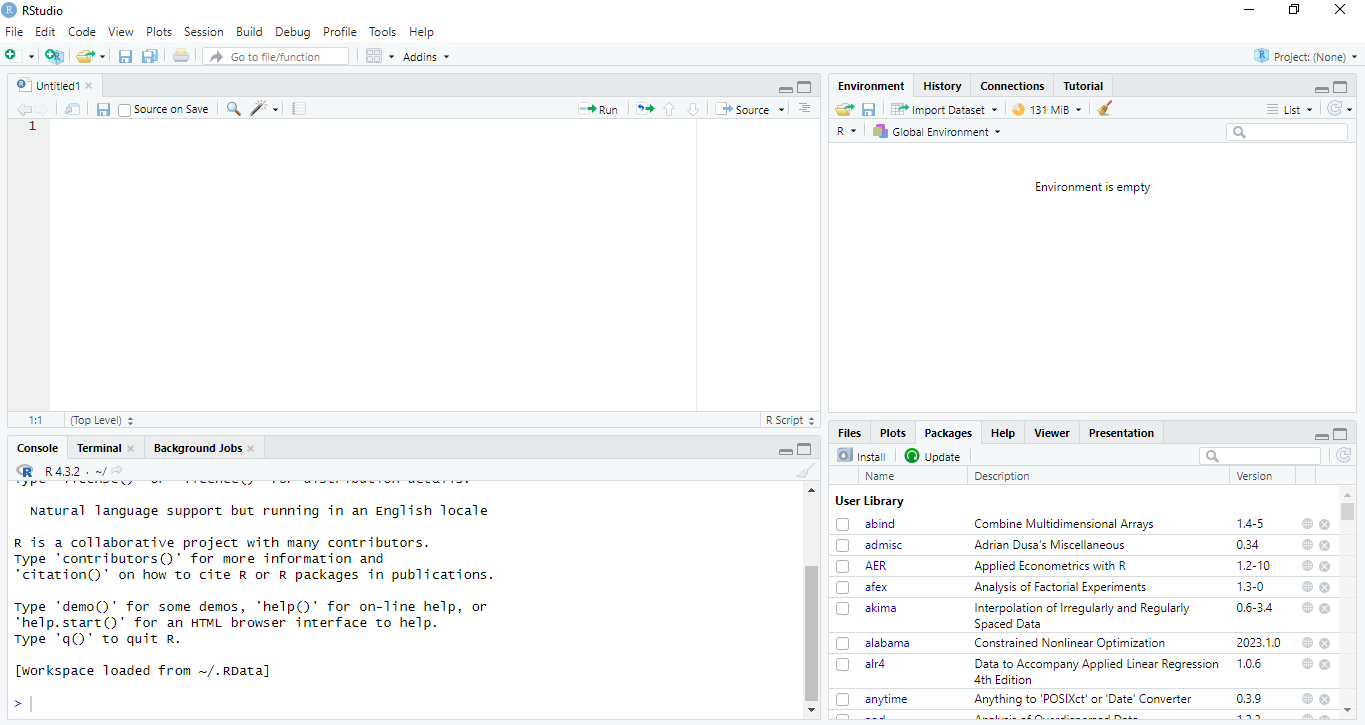
\includegraphics[width=1\linewidth]{figures/4qu} \caption{Antar Muka RStudio dengan Skrip}\label{fig:4qu}
\end{figure}

Skrip ini setara dengan file sintaks di Stata: skrip menyajikan kode yang diperlukan untuk menghasilkan analisis yang diperlukan. Anda dapat menyimpan dan membagikan pekerjaan Anda sebagai skrip yang berisi kode yang dapat dijalankan lain waktu. Hal ini sangat berguna sebagai catatan analisis yang Anda lakukan, melakukan verifikasi analisis atau untuk replikasi studi.

Untuk menjalankan kode dalam skrip R, untuk satu baris kode, letakkan tetikus di depan kode, untuk satu blok baris, pilih kode tersebut, lalu klik tombol \emph{Run} atau tekan \texttt{Ctrl\ +\ Enter} di Windows sistem. Dalam skrip R, dimungkinkan untuk menambahkan komentar menggunakan \#. Segala sesuatu setelah tanda \# akan dianggap sebagai komentar dan tidak akan dijalankan oleh R.

Di awal setiap skrip R, sebaiknya diketikkan paket-paket yang diperlukan untuk mengimplementasikan kode dalam file. Setelah menulis kode untuk memuat paket dengan fungsi \emph{library()}, Anda dapat menambahkan, sebagai komentar, kata kunci untuk mengingatkan tentang penggunaan paket. Ini akan membantu kita mengingat isi file dan menjelaskan kepada orang lain apa yang diperlukan untuk mengimplementasikan kode dalam skrip R.

Ini juga merupakan kebiasan baik untuk mendeskripsikan proyek dan menulis komentar singkat di fungsi-fungsi yang kita buat. Sekali lagi ini berguna bagi penulis skrip dan bagi orang ketiga yang akan membaca kode tersebut.

\hypertarget{manajemen-data-dan-projek-di-r}{%
\section{Manajemen Data dan Projek di R}\label{manajemen-data-dan-projek-di-r}}

R adalah bahasa pemrograman berorientasi objek. Saat Anda membukanya, Anda memiliki lingkungan (\emph{Environment}) kosong yang dapat diisi dengan objek sebanyak kemampuan memori komputer Anda. Segala sesuatu yang ingin Anda simpan atau manipulasi di lain waktu perlu didefinisikan sebagai objek di lingkungan ini. Termasuk disini file data, objek atau hasil model, grafik, dan sebagainya. Artinya, tidak seperti perangkat lunak statistik standar, yang biasanya hanya mengizinkan analis untuk membuka satu kumpulan data, R memungkinkan analis untuk bekerja dengan beberapa file data secara bersamaan.

Ekstensi file R untuk file data adalah .RData. Anda dapat menyimpan satu atau lebih objek dalam file tersebut menggunakan fungsi File \textgreater{} Save (Ctrl + S). Lokasi penyimpanan file ini berada di direktori yang sama dengan file proyek \emph{.Rproj} Anda. Di dalam \emph{RData} tersimpan hasil model, grafik, atau objek yang lain. Hal ini sangat berguna ketika model membutuhkan waktu lama untuk dalam penghitungannya. Hasil tersebut dapat disimpan dan digunakan kembali nanti.

\hypertarget{paket-paket-r}{%
\section{Paket-Paket R}\label{paket-paket-r}}

R bekerja melalui paket-paket (\emph{packages}) termasuk paket dasar dan ribuan paket tambahan. Paket ini mirip dengan aplikasi di ponsel Anda, yang bisa ditambahkan pada ponsel untuk meningkatkan fungsionalitas ponsel Anda. Paket dibuat oleh pengguna dan dibagikan kepada pengguna lain.

Anda perlu mengunduh paket tertentu untuk menyediakan perintah yang diperlukan dan dapat menjalankan model atau analisis tertentu jika fungsi itu tidak tersedia secara \emph{default}. Paket-paket itu memerlukan tiga langkah untuk menggunakannya. Pertama, kita harus menginstal paket itu sendiri, memuatnya dari \emph{library}, dan terakhir memanggil salah satu fungsi paket tersebut.

Paket dapat diunduh di CRAN (\emph{Comprehensive R Archive Network}). Misalnya Anda akan menginstal paket data panel ekonometrik \texttt{plm} (Croissant et al. (\protect\hyperlink{ref-croissantPlmLinearModels2023}{2023})), perintah RStudio berikut akan menginstal paket \texttt{plm} di RStudio versi lokal Anda:

\begin{Shaded}
\begin{Highlighting}[]
\FunctionTok{install.packages}\NormalTok{(}\StringTok{"plm"}\NormalTok{)}
\end{Highlighting}
\end{Shaded}

atau bisa juga melalui opsi drop-down (\emph{Tools -\textgreater{} Install Package}). Paket di CRAN telah dievaluasi untuk memastikan paket tersebut berfungsi di seluruh platform.

Paket bisa juga diinstall dari Github yaitu untuk paket-paket yang tidak terdapat di CRAN. Misalnya Anda akan menginstal paket \texttt{rbbt} (Dunnington (\protect\hyperlink{ref-dunningtonPaleolimbotRbbt2023}{2023})) yaitu konektor R ke \emph{Better Bibtex} untuk \emph{Zotero}. Paket tersebut dapat diinstal menggunakan fungsi \texttt{devtools::install\_\ github} (Wickham et al. (\protect\hyperlink{ref-wickhamDevtoolsToolsMake2022}{2022})). Sebelumnya Anda harus menginstall \texttt{devtools} terlebih dahulu.

\begin{Shaded}
\begin{Highlighting}[]
\FunctionTok{install.packages}\NormalTok{(}\StringTok{"devtools"}\NormalTok{)}
\FunctionTok{require}\NormalTok{(devtools)}
\NormalTok{devtools}\SpecialCharTok{::}\FunctionTok{install\_github}\NormalTok{(}\StringTok{"paleolimbot/rbbt"}\NormalTok{)}
\end{Highlighting}
\end{Shaded}

Sekali sebuah paket sudah diinstal, maka tidak perlu diinstal lagi seperti halnya aplikasi di ponsel Anda. Tetapi perlu diupdate secara rutin karena pengembang paket tersebut mungkin menambahkan fungsionalitas baru. Untuk mengupdate gunakan opsi drop-down (\emph{Tools -\textgreater{} Check for Package Updates}).

RStudio tidak menyimpan paket yang terinstal di memori kerja aktifnya ketika dimatikan. Oleh karena itu, untuk setiap sesi R yang baru, paket yang diperlukan perlu dimuat (\textbf{bukan diinstal ulang, cukup dimuat ulang}) dengan fungsi \texttt{library\ ("nama-paket")} atau \texttt{require("nama-paket")}.

\hypertarget{mengimpor-data-ke-dalam-r}{%
\section{Mengimpor Data ke dalam R}\label{mengimpor-data-ke-dalam-r}}

Dalam praktik analisis data, sering kali data disimpan dalam berbagai format. Selain itu kita mungkin tidak memasukkan data langsung ke R, tetapi menggunakan ke worksheet seperti \emph{Google Sheets} atau bahkan menggunakan program statistik seperti SPSS. R dapat membaca berbagai jenis file data seperti free format text files (txt), comma separated value files (csv), file Excel, file SPSS, file SAS, dan file Stata.

Data yang disimpan dalam file csv dapat diunggah ke RStudio dengan dua cara yang relatif sederhana:

\begin{enumerate}
\def\labelenumi{\arabic{enumi}.}
\tightlist
\item
  Untuk file yang disimpan secara lokal di folder projek pengguna, perintah \texttt{read.csv} akan mengunggah file tersebut. Sebagai contoh, memasukkan perintah berikut akan mengunggah dan menyimpan file csv bernama \emph{inequality.csv} di RStudio:
\end{enumerate}

\begin{Shaded}
\begin{Highlighting}[]
\NormalTok{ineqdata }\OtherTok{\textless{}{-}} \FunctionTok{read.csv}\NormalTok{(}\StringTok{"inequality.csv"}\NormalTok{)}
\end{Highlighting}
\end{Shaded}

Dalam contoh ini, perhatikan sintaksisnya: setelah perintah \texttt{read.csv} dan tanda kurung buka, nama file diberikan di dalam tanda kutip diikuti dengan tanda kurung tutup. Selain itu, data disimpan dengan nama \emph{ineqdata} dengan menggunakan inisial ineqdata \textless-. Data set harus diberi nama sedemikian rupa sehingga dapat direferensikan dalam perintah berikutnya, di mana pilihan nama yang sesuai ditentukan oleh pengguna, bergantung pada konteksnya.

\begin{enumerate}
\def\labelenumi{\arabic{enumi}.}
\setcounter{enumi}{1}
\tightlist
\item
  Jika data dalam format lain, kita perlu menginstal paket untuk mengimpor data misalnya paket \emph{foreign} (Team et al. (\protect\hyperlink{ref-rcoreteamForeignReadData2023}{2023})) yang berfungsi untuk membaca dan menulis file data dari SAS, SPSS dan Stata. Paket ini dapat diinstal dengan perintah \texttt{install.packages("foreign")}. Untuk melakukan impor klik \emph{File \textgreater{} Import Dataset \textgreater{} From Excel, From Stata, From SPSS} dan lain-lain, pilih sesuai jenis data Anda.
\end{enumerate}

\hypertarget{bantuan-tambahan}{%
\section{Bantuan Tambahan}\label{bantuan-tambahan}}

Fitur \emph{Help} di dalam RStudio adalah bagian yang sangat membantu untuk mempelajari cara menggunakan perintah-perintah tertentu di RStudio. Anda sangat disarankan untuk mengeksplorasi lebih lanjut panel \emph{Help} yang terletak di kanan bawah RStudio standar. Selain itu ada banyak rujukan bagus untuk mempelajari R dan RStudio misalnya Crawley (\protect\hyperlink{ref-crawleyBook2012}{2012}), Wickham \& Grolemund (\protect\hyperlink{ref-wickhamDataScience2017}{2017}) dan Verzani (\protect\hyperlink{ref-verzaniGettingStartedRStudio2011}{2011}). Banyak juga rujukan lain yang bisa diakses secara \emph{online}.

\startappendices

\hypertarget{beberapa-rujukan-untuk-belajar-r}{%
\chapter{Beberapa Rujukan untuk Belajar R}\label{beberapa-rujukan-untuk-belajar-r}}

\hypertarget{referensi}{%
\chapter*{Referensi}\label{referensi}}
\addcontentsline{toc}{chapter}{Referensi}

\markboth{Referensi}{}

\hypertarget{refs}{}
\begin{CSLReferences}{1}{0}
\leavevmode\vadjust pre{\hypertarget{ref-crawleyBook2012}{}}%
Crawley, M. J. (2012). \emph{The {R Book}} (2nd edition). {Wiley}.

\leavevmode\vadjust pre{\hypertarget{ref-croissantPlmLinearModels2023}{}}%
Croissant, Y., Millo, G., Tappe, K., Toomet, O., Kleiber, C., Zeileis, A., Henningsen, A., Andronic, L., \& Schoenfelder, N. (2023). \emph{Plm: {Linear Models} for {Panel Data}}.

\leavevmode\vadjust pre{\hypertarget{ref-dalgaardIntroductoryStatistics2008}{}}%
Dalgaard, P. (2008). \emph{Introductory {Statistics} with {R}}. {Springer}. \url{https://doi.org/10.1007/978-0-387-79054-1}

\leavevmode\vadjust pre{\hypertarget{ref-dunningtonPaleolimbotRbbt2023}{}}%
Dunnington, D. (2023). \emph{Paleolimbot/rbbt}.

\leavevmode\vadjust pre{\hypertarget{ref-ismayStatisticalInferenceData2019}{}}%
Ismay, C., \& Kim, A. Y. (2019). \emph{Statistical {Inference} via {Data Science}: {A ModernDive} into {R} and the {Tidyverse}}. {CRC Press}.

\leavevmode\vadjust pre{\hypertarget{ref-rcoreteamLanguageEnvironmentStatistical2023}{}}%
Team, R. C. (2023). \emph{R: {A Language} and {Environment} for {Statistical Computing}}. R Foundation for Statistical Computing.

\leavevmode\vadjust pre{\hypertarget{ref-rcoreteamForeignReadData2023}{}}%
Team, R. C., Bivand, R., Carey, V. J., DebRoy, S., Eglen, S., Guha, R., Herbrandt, S., Lewin-Koh, N., Myatt, M., Nelson, M., Pfaff, B., Quistorff, B., Warmerdam, F., Weigand, S., Foundation, F. S., \& Inc. (2023). \emph{Foreign: {Read Data Stored} by '{Minitab}', '{S}', '{SAS}', '{SPSS}', '{Stata}', '{Systat}', '{Weka}', '{dBase}', ...}

\leavevmode\vadjust pre{\hypertarget{ref-verzaniGettingStartedRStudio2011}{}}%
Verzani, J. (2011). \emph{Getting {Started} with {RStudio}}. {O'Reilly}.

\leavevmode\vadjust pre{\hypertarget{ref-wickhamDataScience2017}{}}%
Wickham, H., \& Grolemund, G. (2017). \emph{R for {Data Science}}. {O'Reilly Media}.

\leavevmode\vadjust pre{\hypertarget{ref-wickhamDevtoolsToolsMake2022}{}}%
Wickham, H., Hester, J., Chang, W., \& Byan, J. (2022). \emph{Devtools: {Tools} to {Make Developing R Packages Easier}}. CRAN.

\end{CSLReferences}

%%%%% REFERENCES


\end{document}
